%!TEX program = xelatex
\documentclass[a4paper,UTF8]{ctexart}
\usepackage[unicode=true,colorlinks,urlcolor=blue,linkcolor=blue,,bookmarksnumbered=true]{hyperref}
\usepackage{latexsym,amssymb,amsmath,amsbsy,amsopn,amstext,amsthm,amsxtra,color,multicol,bm,calc,ifpdf}
\usepackage{graphicx}
\usepackage{diagbox}   % 绘制表格斜线
\usepackage{enumerate}
\usepackage{epstopdf}
\usepackage{fancyhdr}
\usepackage{subfigure}
\usepackage{listings}
\usepackage{multirow}
\usepackage{makeidx}
\usepackage{xcolor} 
\usepackage{fontspec}
\graphicspath{{figures/}}  % 设置图片搜索路径
\theoremstyle{plain} \newtheorem{theorem}{定理}[section]
\theoremstyle{plain} \newtheorem{definition}{定义}[section]
\theoremstyle{plain} \newtheorem{lemma}{引理}[section]
\theoremstyle{plain} \newtheorem{proposition}{命题}[section]
\theoremstyle{plain} \newtheorem{example}{例}[section]
\theoremstyle{plain} \newtheorem{remark}{注}[section]
\theoremstyle{plain} \newtheorem{corollary}{推论}[section]
\newfontfamily\courier{Courier New}
\lstset{linewidth=1.1\textwidth,
        numbers=left, %设置行号位置 
        basicstyle=\small\courier,
        numberstyle=\tiny\courier, %设置行号大小  
        keywordstyle=\color{blue}\courier, %设置关键字颜色  
        %identifierstyle=\bf,
        commentstyle=\it\color[cmyk]{1,0,1,0}\courier, %设置注释颜色 
        stringstyle=\it\color[RGB]{128,0,0}\courier,
        %framexleftmargin=10mm,
        frame=single, %设置边框格式  
        backgroundcolor=\color[RGB]{245,245,244},
        %escapeinside=``, %逃逸字符(1左面的键),用于显示中文  
        breaklines, %自动折行  
        extendedchars=false, %解决代码跨页时,章节标题,页眉等汉字不显示的问题  
        xleftmargin=2em,xrightmargin=2em, aboveskip=1em, %设置边距  
        tabsize=4, %设置tab空格数  
        showspaces=false %不显示空格  
        basicstyle=\small\courier
       }  
\newenvironment{mysolution}{{\color{blue} 解}: }{{\color{magenta}\qed}}
\newcommand\diff{\,{\mathrm d}} % 定义微分d
\newcommand{\p}[3]{\frac{\partial^{#1}#2}{\partial{#3}^{#1}}}  %定义求偏导算子
\newcommand{\ucite}[1]{\textsuperscript{\cite{#1}}}  % 参考文献引用: 上标用 \ucite{ }, 文中用 \cite{ }

\begin{document}
\title{

\includegraphics[width=0.65\textwidth]{onepiece.pdf}\\
\vspace{2em}
\textbf{Softmax 回归学习笔记}}
\author{\emph{李向阳} \quad {\color{blue} d1142845997@gmail.com} }
\date{}


\maketitle
\thispagestyle{empty}

\newpage


\tableofcontents

\newpage

\section{引入}
前面我们介绍了 Logistic 回归模型, 它适用于二分类问题. 如果不只有两个类, 而是有多个类, 那么我们可以将 Logistic 回归模型推广. 多分类的 Logistic 回归又称为 Softmax 回归, 二者都是逻辑回归. 因此, 本次介绍 Softmax 回归模型, 阅读本文之前尽量回顾之前的 Logistic 回归模型.


\section{Softmax 回归模型}

\subsection{数据集}
与 Logistic 回归相同, 我们假设样本是$\{\bm{x}, y\}$, 其中$\bm{x}$表示样本的特征, 设有$n$个特征, 即$\bm{x} = (x_{1}, x_{2}, \cdots, x_{n})^{T}$, 因此我们也可以将样本表示为$\{x_{1}, \cdots, x_{n}, y\}$. 而$y$表示样本的类别, 设总共有$k$个类, 我们用$y = j$表示样本属于第$j$类($j \in \{1, 2, \cdots, k\}$). 我们的目标是由这$n$个样本特征来预测样本的类别. 设训练集有$m$个样本, 即$\{\bm{x}^{(i)}, y^{(i)}\}, i=1,2,\cdots,m$, 其中
\begin{equation*}
\bm{x}^{(i)} = (x_{1}^{(i)},x_{2}^{(i)},\cdots,x_{n}^{(i)})^{T},i = 1,2,\cdots,m
\end{equation*}

仍然提一下记号, 也可以把第$i$个样本表示为$\bm{x}_{i}$, 至于其分量采用双下标来表示, 即有
\begin{equation*}
\bm{x}_{i} = (x_{i1}, x_{i2}, \cdots, x_{in})^{T},i = 1,2,\cdots,m
\end{equation*}

两种方式都可以, 这里我们延续 Logistic 回归的记号, 采用第一种.

\subsection{基本模型}
回想一下, 实际上 Logistic 回归模型的假设函数是样本属于正类的概率. 所谓 Softmax 回归模型, 其实道理一样, 对于给定的样本$\bm{x}$, 我们想用假设函数针对每一个类别$j$估算出概率值$p(y = j | \bm{x})$, 也就是估计出$\bm{x}$的每一种分类结果可能出现的概率. 因此, 我们的假设函数将要输出一个$k$维的向量(向量元素的和为$1$)来表示这$k$个概率的估计值. 具体地说, 我们的假设函数$h_{\bm{\theta}}(\bm{x})$形式如下:
$$
h_{\bm{\theta}}(\bm{x}) = 
\begin{bmatrix}
p(y = 1 | \bm{x}; \bm{\theta}) \\ 
p(y = 2 | \bm{x}; \bm{\theta}) \\ 
\vdots \\ 
p(y = k | \bm{x}; \bm{\theta})
\end{bmatrix}
= \frac{1}{\sum_{l=1}^{k} e^{\bm{\theta}_{l}^T \bm{x}}}
\begin{bmatrix}
e^{\bm{\theta}_{1}^T \bm{x}} \\ 
e^{\bm{\theta}_{2}^T \bm{x}} \\ 
\vdots \\ 
e^{\bm{\theta}_{k}^T \bm{x}}
\end{bmatrix}
$$

其中$\bm{\theta}_1, \bm{\theta}_2, \cdots, \bm{\theta}_k \in \mathbb{R}^{n+1}$是模型的参数. 注意同 Logistic 回归一样, 为了记号的方便, 引入$x_{0} = 1$, 即有$\bm{x} = (x_{0}, x_{1}, \cdots, x_{n})^{T}$. 注意到$\frac{1}{\sum_{l=1}^{k} e^{\bm{\theta}_l^T \bm{x}}}$这一项起到了归一化的作用, 使得所有概率之和为$1$.

为了方便起见, 我们用$\bm{\theta}$来表示全部的模型参数(本来最好使用大写). 由于$\bm{\theta}_1, \cdots, \bm{\theta}_k$每个都是$n+1$维的向量, 所以我们把$\bm{\theta}_1, \cdots, \bm{\theta}_k$按行并起来, 也就是说实际上$\bm{\theta}$是一个$k \times (n+1)$的矩阵, 如下所示
$$
\bm{\theta} = 
\begin{bmatrix}
\bm{\theta}_{1}^{T} \\ 
\bm{\theta}_{2}^{T} \\ 
\vdots \\ 
\bm{\theta}_{k}^{T}
\end{bmatrix}
$$


\subsection{参数估计}
同 Logistic 回归一样, 我们仍然是把样本集的似然函数取负号作为代价函数, 然后通过极小化代价函数来求得参数估计值.

对于一个样本$\{\bm{x}, y\}$, 我们知道它属于第$j$类的概率为
\begin{equation*}
p(y = j | \bm{x}; \bm{\theta}) = \frac{e^{\bm{\theta}_{j}^T \bm{x}}}{\sum_{l=1}^{k} e^{\bm{\theta}_{l}^T \bm{x}}}
\end{equation*}

其实挺类似于$0-1$分布的(上式相当于概率分布列), 其概率(分布)函数为
\begin{align*}
p(y | \bm{x}; \bm{\theta}) & = p(y = 1 | \bm{x}; \bm{\theta})^{1\{y=1\}} \cdot p(y = 2 | \bm{x}; \bm{\theta})^{1\{y=2\}} \cdots p(y = k | \bm{x}; \bm{\theta})^{1\{y=k\}} \\ 
& = \prod_{j=1}^{k} p(y = j | \bm{x}; \bm{\theta})^{1\{y=j\}}
\end{align*}

其中$1\{\cdot\}$是示性函数, 大括号里的表达式为真时取为$1$, 否则取为$0$. 嗯, 确实很像$0-1$分布的概率函数的构造啊!

由于假定$m$个样本独立同分布, 因此似然函数为
\begin{equation*}
L(\bm{\theta}) = \prod_{i=1}^{m} p(y^{(i)} | \bm{x}^{(i)}; \bm{\theta}) = \prod_{i=1}^{m} \prod_{j=1}^{k} p(y^{(i)} = j | \bm{x}^{(i)}; \bm{\theta})^{1\{y^{(i)}=j\}}
\end{equation*}

其对数似然函数为
\begin{align*}
\ell (\bm{\theta}) & = \ln L(\bm{\theta}) = \sum_{i=1}^{m} \ln p(y^{(i)} | \bm{x}^{(i)}; \bm{\theta}) \\ 
& = \sum_{i=1}^{m} \ln \prod_{j=1}^{k} p(y^{(i)} = j | \bm{x}^{(i)}; \bm{\theta})^{1\{y^{(i)}=j\}} \\ 
& = \sum_{i=1}^{m} \sum_{j=1}^{k} 1\{y^{(i)}=j\} \ln p(y^{(i)} = j | \bm{x}^{(i)}; \bm{\theta}) \\ 
& = \sum_{i=1}^{m} \sum_{j=1}^{k} 1\{y^{(i)}=j\} \ln \frac{e^{\bm{\theta}_{j}^T \bm{x}^{(i)}}}{\sum_{l=1}^{k} e^{\bm{\theta}_{l}^T \bm{x}^{(i)}}}
\end{align*}

因此, 我们的代价函数构造为
\begin{equation*}
J(\bm{\theta}) = - \frac{1}{m} \left( \sum_{i=1}^{m} \sum_{j=1}^{k} 1\{y^{(i)}=j\} \ln \frac{e^{\bm{\theta}_{j}^T \bm{x}^{(i)}}}{\sum_{l=1}^{k} e^{\bm{\theta}_{l}^T \bm{x}^{(i)}}} \right)
\end{equation*}

值得注意的是, 上述公式是 Logistic 回归代价函数的推广. 回想一下, 其实 Logistic 回归代价函数可以改为
\begin{align*}
J(\bm{\theta}) & = - \frac{1}{m} \left( \sum_{i=1}^{m} (1 - y^{(i)}) \ln (1 - h_{\bm{\theta}}(\bm{x}^{(i)})) + y^{(i)} \ln h_{\bm{\theta}}(\bm{x}^{(i)}) \right) \\ 
& = - \frac{1}{m} \left( \sum_{i=1}^{m} \sum_{j=0}^{1} 1\{y^{(i)}=j\} \ln p(y^{(i)} = j | \bm{x}^{(i)}; \bm{\theta}) \right)
\end{align*}

当时是用$y=1$和$y=0$区分正负类, 现在是用$y=1,2,\cdots,k$表示$k$个类, 因此 Softmax 损失函数中对类标记的$k$个可能值进行了累加.

接下来通过最小化$J(\bm{\theta})$来求得参数$\bm{\theta}$. 当然, 还是需要借助优化算法, 比如梯度下降法、牛顿法、拟牛顿法等等. 不管怎么样, 求梯度是无法避免的. 现在我们来求一下梯度(偏导数).

我们知道参数$\bm{\theta}$是一个矩阵, 是由向量$\bm{\theta}_1, \cdots, \bm{\theta}_k$按行并起来的, 所以为了求导的方便, 我们也是分别对向量$\bm{\theta}_1, \cdots, \bm{\theta}_k$求偏导, 其实计算并不难, 比如计算对向量$\bm{\theta}_{j}$的导数, 由于
\begin{align*}
J(\bm{\theta}) & = - \frac{1}{m} \left( \sum_{i=1}^{m} \sum_{j=1}^{k} 1\{y^{(i)}=j\} \ln \frac{e^{\bm{\theta}_{j}^T \bm{x}^{(i)}}}{\sum_{l=1}^{k} e^{\bm{\theta}_{l}^T \bm{x}^{(i)}}} \right) \\ 
& = - \frac{1}{m} \left( \sum_{i=1}^{m} \sum_{j=1}^{k} 1\{y^{(i)}=j\} \left( \ln (e^{\bm{\theta}_{j}^T \bm{x}^{(i)}}) - \ln \left( \sum_{l=1}^{k} e^{\bm{\theta}_{l}^T \bm{x}^{(i)}} \right) \right) \right) \\ 
& = - \frac{1}{m} \left( \sum_{i=1}^{m} \sum_{j=1}^{k} 1\{y^{(i)}=j\} \left( \bm{\theta}_{j}^T \bm{x}^{(i)} - \ln \left( \sum_{l=1}^{k} e^{\bm{\theta}_{l}^T \bm{x}^{(i)}} \right) \right) \right) \\
& = - \frac{1}{m} \large( \sum_{i=1}^{m} ( 1\{y^{(i)}=1\} \cdot \bm{\theta}_{1}^T \bm{x}^{(i)} + \cdots +  1\{y^{(i)}=k\} \cdot \bm{\theta}_{k}^T \bm{x}^{(i)}  \\ 
& \qquad \qquad - \left[ 1\{y^{(i)}=1\} + \cdots + 1\{y^{(i)}=k\} \right] \cdot \ln \sum_{l=1}^{k} e^{\bm{\theta}_{l}^T \bm{x}^{(i)}} ) \large) \\ 
& = - \frac{1}{m} \left( \sum_{i=1}^{m} \left( 1\{y^{(i)}=1\} \cdot \bm{\theta}_{1}^T \bm{x}^{(i)} + \cdots + 1\{y^{(i)}=k\} \cdot \bm{\theta}_{k}^T \bm{x}^{(i)}  - \ln \left( \sum_{l=1}^{k} e^{\bm{\theta}_{l}^T \bm{x}^{(i)}} \right) \right) \right)
\end{align*}

最后一步是因为$[1\{y^{(i)}=1\} + \cdots 1\{y^{(i)}=k\}]$的结果肯定是$1$. 于是可得
\begin{align*}
\nabla_{\bm{\theta}_{j}} J(\bm{\theta}) & = - \frac{1}{m} \left( \sum_{i=1}^{m} \left( 1\{y^{(i)}=j\} \cdot \bm{x}^{(i)} - \frac{e^{\bm{\theta}_{j}^T \bm{x}^{(i)}}}{\sum_{l=1}^{k} e^{\bm{\theta}_{l}^T \bm{x}^{(i)}}} \cdot \bm{x}^{(i)} \right) \right) \\ 
& = - \frac{1}{m} \left( \sum_{i=1}^{m} \bm{x}^{(i)} \left( 1\{y^{(i)}=j\} - \frac{e^{\bm{\theta}_{j}^T \bm{x}^{(i)}}}{\sum_{l=1}^{k} e^{\bm{\theta}_{l}^T \bm{x}^{(i)}}} \right) \right) \\ 
& = - \frac{1}{m} \left( \sum_{i=1}^{m} \bm{x}^{(i)} \left( 1\{y^{(i)}=j\} - p(y^{(i)} = j | \bm{x}^{(i)}; \bm{\theta}) \right) \right)
\end{align*}

这就是偏导数的表达式了. 注意$\nabla_{\bm{\theta}_{j}} J(\bm{\theta})$ 本身也是一个向量, 它的第$l$个元素$\p{}{J(\bm{\theta})}{\theta_{jl}}$是$J(\bm{\theta})$对$\bm{\theta}_{j}$的第$l$个分量的偏导数. 有了偏导数, 便可以使用优化算法了, 比如梯度下降法
\begin{equation*}
\bm{\theta}_{j} := \bm{\theta}_{j} - \alpha \nabla_{\bm{\theta}_{j}} J(\bm{\theta}), j = 1,2,\cdots,k
\end{equation*}


\subsection{参数特点}
Softmax 回归有一个不寻常的特点, 它的参数集其实是“冗余”的. 很简单, 由于概率之和为$1$, 所以知道了样本属于前$k-1$类的概率, 自然就知道了样本属于第$k$类的概率, 因此用不着引入$k$个参数向量, 只需要引入$k-1$个即可. 我们还可以通过如下方式来阐述这一特点: 假设我们从每个参数向量$\bm{\theta}_{j}$中都减去一个向量$\bm{\psi}$, 这时每一个$\bm{\theta}_{j}$都变成了$\bm{\theta}_{j} - \bm{\psi}(j=1,\cdots,k)$, 此时假设函数中样本分类的概率变为下式
\begin{align*}
p(y = j | \bm{x}; \bm{\theta}) & = \frac{e^{(\bm{\theta}_{j} - \bm{\psi})^T \bm{x}}}{\sum_{l=1}^{k} e^{(\bm{\theta}_{l} - \bm{\psi})^T \bm{x}}} \\ 
& = \frac{e^{\bm{\theta}_{j}^{T} \bm{x}}  e^{- \bm{\psi}^T \bm{x}}}{\sum_{l=1}^{k} e^{\bm{\theta}_{l}^{T} \bm{x}}  e^{- \bm{\psi}^T \bm{x}}} \\ 
& = \frac{e^{\bm{\theta}_{j}^{T} \bm{x}} }{\sum_{l=1}^{k} e^{\bm{\theta}_{l}^{T} \bm{x}} } 
\end{align*}

可以看到, 从$\bm{\theta}_{j}$中减去$\bm{\psi}$完全不影响假设函数的预测结果! 这就表明 Softmax 回归模型中存在冗余的参数. 换句话说, 对于任意一个用于拟合数据的假设函数, 可以求出多组参数值, 这些参数得到的是完全相同的假设函数$h_{\bm{\theta}}(\bm{x})$.

进一步而言, 如果参数$(\bm{\theta}_1, \bm{\theta_2}, \cdots, \bm{\theta}_k)$是代价函数$J(\bm{\theta})$的极小值点, 那么$(\bm{\theta}_1 - \bm{\psi}, \bm{\theta}_2 - \bm{\psi}, \cdots, \bm{\theta}_k - \bm{\psi})$同样也是它的极小值点, 其中$\bm{\psi}$可以为任意向量, 因此使$J(\bm{\theta})$最小化的解是不唯一的, 不过这些解的分类结果是相同的. (有趣的是, 由于$J(\bm{\theta})$仍然是一个凸函数, 因此梯度下降时不会遇到局部最优解的问题. 但是 Hessian 矩阵是奇异的/不可逆的, 这会直接导致采用牛顿法优化就遇到数值计算的问题)

注意, 当$\bm{\psi} = \bm{\theta}_{k}$时, 我们总可以将$\bm{\theta}_{k}$替换为$\bm{\theta}_{k} - \bm{\psi} = \bm{0}$(即替换为全零向量), 并且这种变换不会影响假设函数. 因此我们可以去掉参数向量$\bm{\theta}_{k}$(或者其他$\bm{\theta}_{j}$中的任意一个)而不影响假设函数的表达能力. 实际上, 与其优化全部的$k \times (n+1)$个参数$(\bm{\theta}_1, \bm{\theta}_2, \cdots, \bm{\theta}_k)$(其中$\bm{\theta}_{j} \in \mathbb{R}^{n+1}$), 我们可以令$\bm{\theta}_{k} = \bm{0}$, 只优化剩余的$(k-1) \times (n+1)$个参数, 这样算法依然能够正常工作. 也因此, 有些文献书籍中直接把 Softmax 回归模型写成
\begin{align*}
p(y = j | \bm{x}; \bm{\theta}) & = \frac{e^{\bm{\theta}_{j}^{T} \bm{x} }} {1 + \sum_{l=1}^{k-1} e^{\bm{\theta}_{l}^{T} \bm{x} }} , j = 1, 2, \cdots, k-1 \\ 
p(y = k | \bm{x}; \bm{\theta}) & = \frac{1} {1 + \sum_{l=1}^{k-1} e^{\bm{\theta}_{l}^{T} \bm{x} }}
\end{align*}

然而在实际应用中, 为了算法实现更简单清楚, 往往会保留所有参数$(\bm{\theta}_1, \bm{\theta}_2, \cdots, \bm{\theta}_k)$, 而不是任意的将某一参数设置为全零向量. 

此外, 我们还需要在代价函数中加入参数惩罚项(也称权重衰减项)来正则化. 也就是代价函数变成
\begin{equation*}
J(\bm{\theta}) = - \frac{1}{m} \left( \sum_{i=1}^{m} \sum_{j=1}^{k} 1\{y^{(i)}=j\} \ln \frac{e^{\bm{\theta}_{j}^T \bm{x}^{(i)}}}{\sum_{l=1}^{k} e^{\bm{\theta}_{l}^T \bm{x}^{(i)}}} \right) + \frac{\lambda}{2} \sum_{i=1}^{k} \sum_{j=0}^{n} \theta_{ij}^{2}
\end{equation*}

有了这个权重衰减项以后($\lambda > 0$), 代价函数还变成了严格的凸函数, 这样就可以保证得到唯一的解了. 此时的 Hessian 矩阵变为可逆矩阵, 并且因为$J(\bm{\theta})$是凸函数, 梯度下降法和 BFGS 等算法可以保证收敛到全局最优解.

当然, 这个新代价函数的导数是比较容易计算的, 如下
\begin{equation*}
\nabla_{\bm{\theta}_{j}} J(\bm{\theta}) = - \frac{1}{m} \left( \sum_{i=1}^{m} \bm{x}^{(i)} \left( 1\{y^{(i)}=j\} - p(y^{(i)} = j | \bm{x}^{(i)}; \bm{\theta}) \right) \right) + \lambda \bm{\theta}_{j}
\end{equation*}


\subsection{模型比较}
\subsubsection{Softmax 回归与 Logistic 回归的关系}
我们说 Softmax 回归是 Logistic 回归的推广. 特别的, 当类别数$k=2$时, Softmax 回归就退化为 Logistic 回归. 这表明, Softmax 回归是 Logistic 回归的一般形式. 具体的说, 当$k=2$时, Softmax 回归的假设函数为
$$
h_{\bm{\theta}}(\bm{x}) = \frac{1}{e^{\bm{\theta}_{1}^{T} \bm{x}} + e^{\bm{\theta}_{2}^{T} \bm{x}}} 
\begin{bmatrix}
e^{\bm{\theta}_{1}^{T} \bm{x}} \\ 
e^{\bm{\theta}_{2}^{T} \bm{x}} 
\end{bmatrix}
$$

利用 Softmax 回归参数冗余的特点, 我们另$\bm{\psi} = \bm{\theta}_1$, 并从两个参数向量中都减去向量$\bm{\theta}_1$, 得到
\begin{align*}
h_{\bm{\theta}}(\bm{x}) & = \frac{1}{e^{\bm{0}^{T} \bm{x}} + e^{(\bm{\theta}_{2} -  \bm{\theta}_{1})^{T} \bm{x}}} 
\begin{bmatrix}
e^{\bm{0}^{T} \bm{x}} \\ 
e^{(\bm{\theta}_{2} -  \bm{\theta}_{1})^{T} \bm{x}} 
\end{bmatrix} 
=
\frac{1}{1 + e^{(\bm{\theta}_{2} -  \bm{\theta}_{1})^{T} \bm{x}}} 
\begin{bmatrix}
1 \\ 
e^{(\bm{\theta}_{2} -  \bm{\theta}_{1})^{T} \bm{x}} 
\end{bmatrix} \\ 
& = 
\begin{bmatrix}
\frac{1}{1 + e^{(\bm{\theta}_{2} -  \bm{\theta}_{1})^{T} \bm{x}}} \\ 
\frac{e^{(\bm{\theta}_{2} -  \bm{\theta}_{1})^{T} \bm{x}}} {1 + e^{(\bm{\theta}_{2} -  \bm{\theta}_{1})^{T} \bm{x}}} 
\end{bmatrix}
=
\begin{bmatrix}
\frac{1}{1 + e^{(\bm{\theta}_{2} -  \bm{\theta}_{1})^{T} \bm{x}}} \\ 
1 -  \frac{1}{1 + e^{(\bm{\theta}_{2} -  \bm{\theta}_{1})^{T} \bm{x}}}
\end{bmatrix}
\end{align*}

因此, 若用$\bm{\beta}$来表示$\bm{\theta}_{2} - \bm{\theta}_{1}$, 我们就会发现 Softmax 回归预测其中一个类别的概率为$\frac{1}{1 + e^{\bm{\beta}^{T} \bm{x} }}$, 另一个类的概率为$1 - \frac{1}{1 + e^{\bm{\beta}^{T} \bm{x} }}$, 这与 Logistic 回归是一致的.


\subsubsection{Softmax 回归 VS $k$个二元分类器}
如果我们在开发一个音乐分类的应用, 需要对$k$种类型的音乐进行识别, 那么是选择使用 Softmax 分类器, 还是使用 Logistic 回归算法建立$k$个独立的二元分类器呢?

这一选择取决于音乐的类别之间是否互斥, 例如, 如果有四个类别的音乐, 分别为: 古典音乐、乡村音乐、摇滚乐和爵士乐, 那么我们可以假设每个训练样本只会被打上一个标签(即: 一首歌只能属于这四种音乐类型的其中一种), 此时应该使用类别数$k=4$的Softmax回归. (如果在我们的数据集中, 有的歌曲不属于以上四类的其中任何一类, 那么我们可以添加一个“其他类”, 并将类别数$k$设为$5$)

如果我们的四个类别如下: 人声音乐、舞曲、影视原声、流行歌曲, 那么这些类别之间并不是互斥的. 例如一首歌曲可以来源于影视原声, 同时也包含人声. 这种情况下, 使用$4$个二分类的 Logistic 回归分类器更为合适. 这样, 对于每个新的音乐作品, 我们的算法可以分别判断它是否属于各个类别.



\section{编程计算}
真正编程计算时, 我们需要充分利用向量化的思想. 本系列讲述每个算法时所用的编程语言不太一样, 不过就$3$种, 有 Matlab, Python 和 R 语言. 至于本文, 主要用的是 Matlab, 采用的数据集是著名的 MNIST 手写数字识别集, 训练样本有$m=60000$个, 每个样本都对应$0-9$中的一个数, 也就是说总共有$k=10$类.为了方便, 我们把数字$0$看成是第$10$类. 由于把图片转化为了$28 \times 28$的灰度矩阵, 并把它拉直为了向量, 因此这里的特征变量数$n=784$.

编程中很关键的是代价函数和导数的计算. 这里粗略的介绍一下.

我们的样本数据是$\mathrm{data} = [\bm{x}^{(1)}, \bm{x}^{(2)}, \cdots, \bm{x}^{(m)}]$, 也就是 data 是一个$n \times m$的矩阵. 我们的参数$\bm{\theta}$也是一个矩阵, 上面已经提过了.

可以看到代价函数中出现了$1\{y^{(i)} = j\}$, 因此为了方便计算, 定义一个矩阵, 称为 ground truth matrix (或 indicator response matrix), 不妨记为$M$, 其元素为$M(j, i) = 1\{y^{(i)} = j\}$, 相当于$j$表示类别, 为行数, $i$代表样本, 为列数, 也就是说$M$是一个$k \times m$的矩阵, 记录了每个训练样本的真实类别, 直观的看, 就是如下图\ref{ground}一个大矩阵
\begin{figure}[!htb]
	\centering
	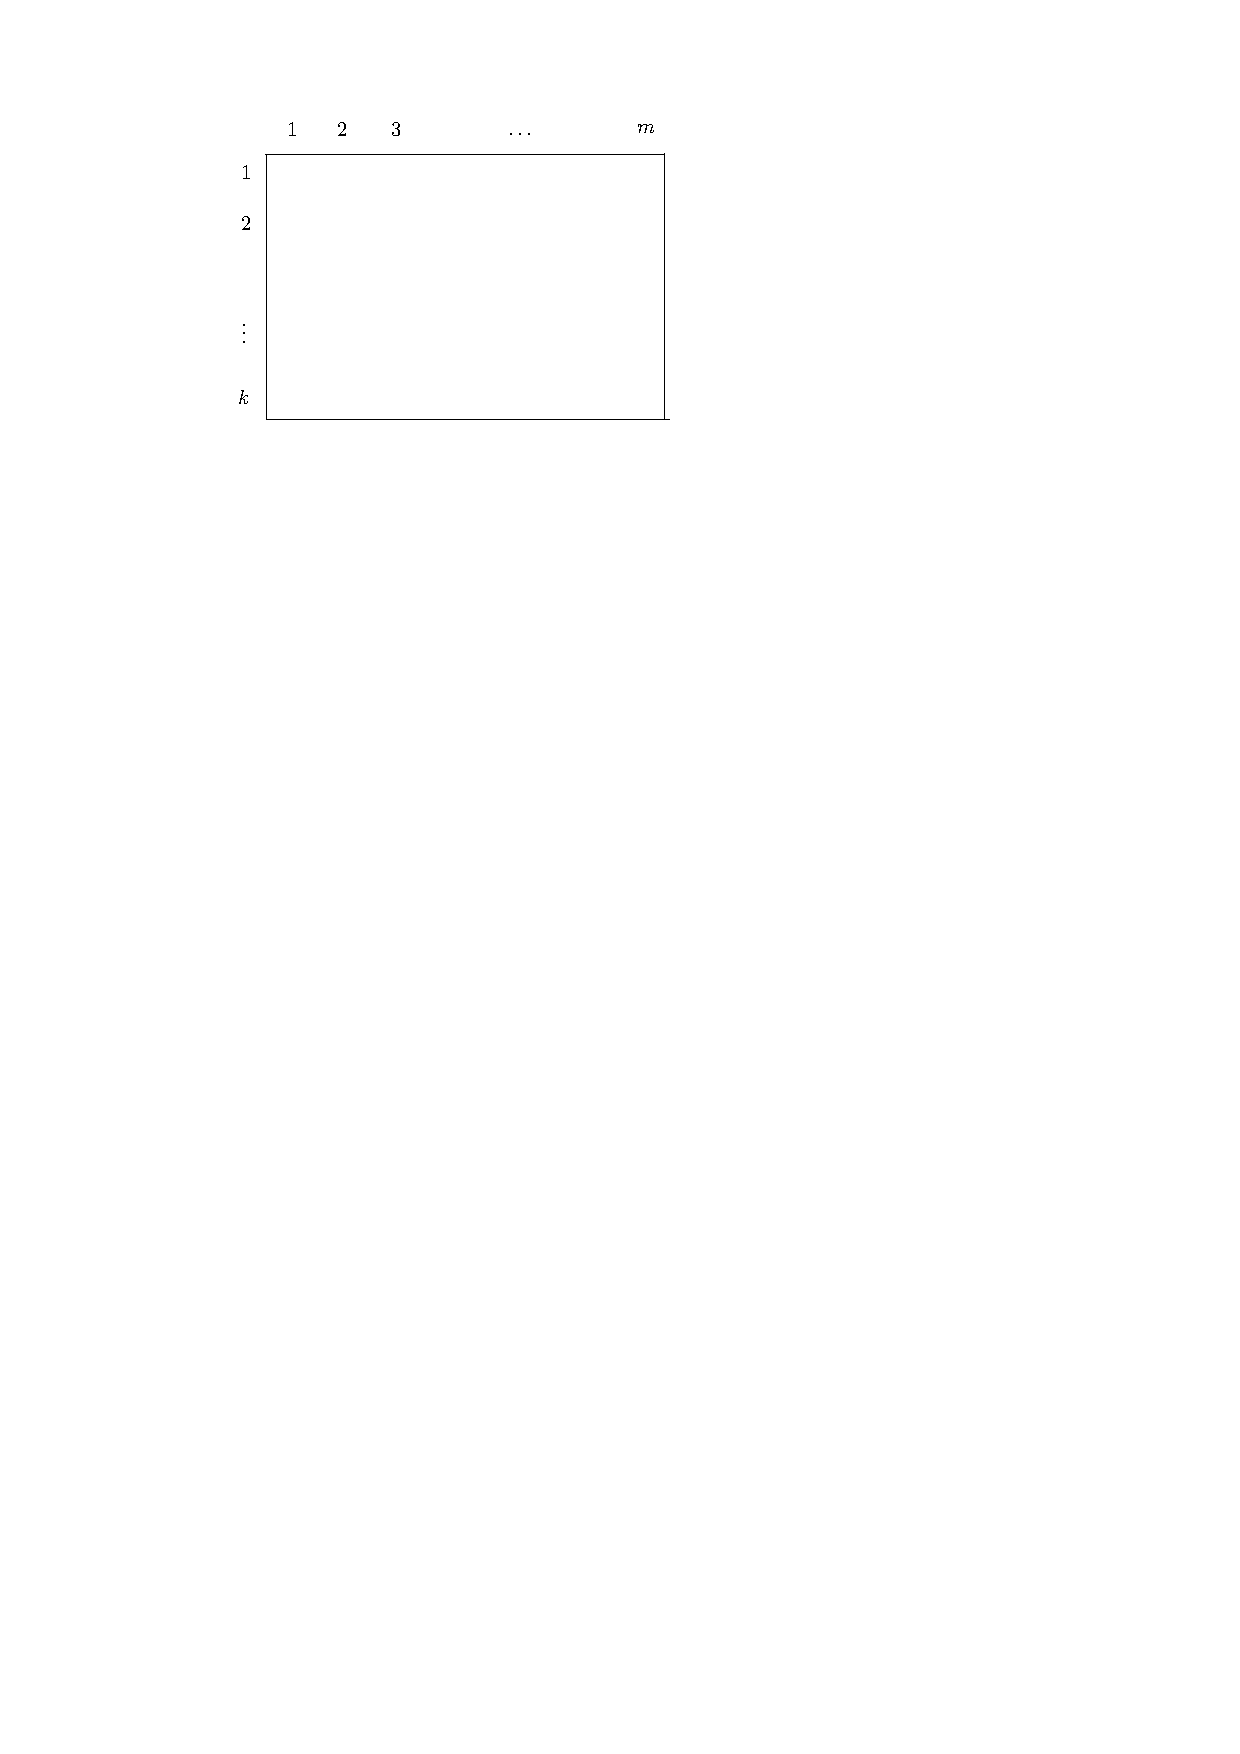
\includegraphics[width = 0.75 \textwidth]{ground.pdf}
	\caption{ground truth matrix}
	\label{ground}
\end{figure}

对于每一列来看, 比如第$i$列, 其实就表示第$i$个样本属于哪一类, 如果属于第$j$类就把对应的第$j$行的元素填成$1$, 然后该列的其它元素默认全填成$0$. 用 Matlab 生成这样一个矩阵很简单, 只需要如下一条语句即可
\begin{lstlisting}[language=matlab]
M = full(sparse(labels, 1:m, 1))
\end{lstlisting}

命令 M = sparse(r, c, v) 会产生一个稀疏矩阵, 其元素为 M(r(i), c(i)) = v(i), 其中 r 与 v 都是一个向量, 未指定位置的元素默认全为$0$. 如果不理解为什么这条命令产生的是我们需要的 ground truth matrix 的话, 让$i=1,2,\cdots, m$代进去就理解了.

显然, 两个矩阵$\bm{\theta}$与 data 的乘积为
$$
\bm{\theta} \cdot \mathrm{data} = 
\begin{bmatrix}
\bm{\theta}_{1}^{T} \\ 
\bm{\theta}_{2}^{T} \\ 
\vdots \\ 
\bm{\theta}_{k}^{T}
\end{bmatrix}
[\bm{x}^{(1)}, \bm{x}^{(2)}, \cdots, \bm{x}^{(m)}] = 
\begin{bmatrix}
\bm{\theta}_{1}^{T} \bm{x}^{(1)} & \bm{\theta}_{1}^{T} \bm{x}^{(2)} & \cdots & \bm{\theta}_{1}^{T} \bm{x}^{(m)} \\ 
\bm{\theta}_{2}^{T} \bm{x}^{(1)} & \bm{\theta}_{2}^{T} \bm{x}^{(2)} & \cdots & \bm{\theta}_{2}^{T} \bm{x}^{(m)} \\ 
\vdots & \vdots & \ddots & \vdots \\ 
\bm{\theta}_{k}^{T} \bm{x}^{(1)} & \bm{\theta}_{k}^{T} \bm{x}^{(2)} & \cdots & \bm{\theta}_{k}^{T} \bm{x}^{(m)}
\end{bmatrix}
$$

得到这个矩阵后, 利用 Matlab 中的 bsxfun 函数(感觉类似于 R 中的 apply 系列函数, 重要性和用法不必多说了)可以很轻松的得到概率矩阵(下面把$p(y^{(i)} = j | \bm{x}^{(i)}; \bm{\theta})$简写为了$p(y^{(i)} = j)$)
$$
p = 
\begin{bmatrix}
p(y^{(1)} = 1) & p(y^{(2)} = 1) & \cdots & p(y^{(1)} = 1) \\ 
p(y^{(1)} = 2) & p(y^{(2)} = 2) & \cdots & p(y^{(1)} = 2) \\
\vdots & \vdots & \ddots & \vdots \\ 
p(y^{(1)} = k) & p(y^{(2)} = k) & \cdots & p(y^{(1)} = k)
\end{bmatrix}
$$

把概率矩阵用$\ln$作用一下, 记为$P = \ln p$, 阶数仍为$k \times m$, 仔细观察一下, 代价函数中的那个双$\sum$求和不正是$\sum\limits_{i=1}^{m} \sum\limits_{j=1}^{k} M_{ji} \cdot P_{ji}$吗?

也就是说其实就是把矩阵$M$和$P$的对应元素相乘, 然后再求所有元素的和即可. 这直接使用 Matlab 中的“.*”号然后再用 sum 函数作用两次就可以了, 当然, 也可以把矩阵拉直为向量做, 如下语句
\begin{lstlisting}[language=matlab]
cost = -1 / m * M(:)' * log(p(:)) + lambda / 2 * sum(theta(:) .^ 2);
\end{lstlisting}

至此, 代价函数的计算就完成了.

再来看导数的计算. 为了方便, 我们定义一个偏导数矩阵, 记为 thetagrad, 就是$J(\bm{\theta})$对参数矩阵$\bm{\theta}$的每个分量的偏导数, 其实也就是相应地把梯度向量$\nabla_{\bm{\theta}_{j}} J(\bm{\theta}) (j=1,2,\cdots,k)$按行并起来
$$
\mathrm{thetagrad} = 
\begin{bmatrix}
(\nabla_{\bm{\theta}_{1}} J(\bm{\theta}))^{T} \\ 
(\nabla_{\bm{\theta}_{2}} J(\bm{\theta}))^{T} \\
\vdots \\ 
(\nabla_{\bm{\theta}_{k}} J(\bm{\theta}))^{T} 
\end{bmatrix}
$$

而我们知道
\begin{align*}
\nabla_{\bm{\theta}_{j}} J(\bm{\theta}) & = - \frac{1}{m} \left( \sum_{i=1}^{m} \bm{x}^{(i)} \left( 1\{y^{(i)}=j\} - p(y^{(i)} = j | \bm{x}^{(i)}; \bm{\theta}) \right) \right) + \lambda \bm{\theta}_{j} \\ 
& = - \frac{1}{m} \left( \sum_{i=1}^{m} \bm{x}^{(i)} \left( M_{ji} - p_{ji} \right) \right) + \lambda \bm{\theta}_{j}
\end{align*}

于是可得
\begin{align*}
\mathrm{thetagrad} & = 
\begin{bmatrix}
(\nabla_{\bm{\theta}_{1}} J(\bm{\theta}))^{T} \\ 
(\nabla_{\bm{\theta}_{2}} J(\bm{\theta}))^{T} \\
\vdots \\ 
(\nabla_{\bm{\theta}_{k}} J(\bm{\theta}))^{T} 
\end{bmatrix} \\ 
& = 
- \frac{1}{m} 
\begin{bmatrix}
\sum_{i=1}^{m} (M_{1i} - p_{1i}) \cdot (\bm{x}^{(i)})^{T} \\ 
\sum_{i=1}^{m} (M_{2i} - p_{2i}) \cdot (\bm{x}^{(i)})^{T} \\
\vdots \\ 
\sum_{i=1}^{m} (M_{ki} - p_{ki}) \cdot (\bm{x}^{(i)})^{T} \\
\end{bmatrix}
+ \lambda 
\begin{bmatrix}
\bm{\theta}_{1}^{T} \\ 
\bm{\theta}_{2}^{T} \\ 
\vdots \\ 
\bm{\theta}_{k}^{T}
\end{bmatrix} \\ 
& = - \frac{1}{m} 
\begin{bmatrix}
M_{11} - p_{11} & M_{12} - p_{12}  & \cdots & M_{1m} - p_{1m} \\ 
M_{21} - p_{21} & M_{22} - p_{22}  & \cdots & M_{2m} - p_{2m} \\ 
\vdots & \vdots & \ddots & \vdots \\ 
M_{k1} - p_{k1} & M_{k2} - p_{k2}  & \cdots & M_{km} - p_{km}
\end{bmatrix} 
\begin{bmatrix}
(\bm{x}^{(1)})^{T} \\ 
(\bm{x}^{(2)})^{T} \\ 
\vdots \\ 
(\bm{x}^{(m)})^{T}
\end{bmatrix}
+ \lambda \bm{\theta} \\ 
& = - \frac{1}{m} (M - p) \cdot \mathrm{data}^{T} + \lambda \bm{\theta}
\end{align*}

其中$M, p, \mathrm{data}, \bm{\theta}$都是矩阵. 因此计算 thetagrad 只需要一条语句即可
\begin{lstlisting}[language = matlab]
thetagrad = -1 / m * (M - p) * data' + lambda * theta;
\end{lstlisting}

这里先说这么多, 关于编程的更多细节直接看程序即可.



\section{总结}

\subsection{参考资料}
\begin{enumerate}[(1)]
\item Andrew Ng 的 Ufldl: \url{http://deeplearning.stanford.edu/wiki/index.php/Softmax%E5%9B%9E%E5%BD%92}, 本文的内容基本来自于此.

对应的编程练习页面在 \url{http://deeplearning.stanford.edu/wiki/index.php/Exercise:Softmax_Regression}, 里面有一些编程的 Tips 和 程序文件, 不过程序有一小部分是需要自己完成的, 我是参考了 Github 上的 \url{https://github.com/zellyn/deeplearning-class-2011/tree/master/ufldl/library}, 这个 Repository 是深度学习, 其中包含了 Ufldl 几乎全部的编程解答.

Andrew Ng 的 Ufldl 好像有多个版本, 我还看了这个 \url{http://ufldl.stanford.edu/tutorial/supervised/SoftmaxRegression/}, 这个系列也不错, 只是没有中文翻译而已, 其对应的也有编程练习, 解答在 Github 中也有一个: \url{https://github.com/amaas/stanford_dl_ex}.

总之, 这两个 Ufldl 系列都很不错, 因为也涉及了其他算法, 值得阅读.

此外, 他的公开课的 Notes 中有一节讲述了如何构造 GLM 模型, 其中就包含了 Softmax 模型是怎么来的, 非常不错.

\item MNIST 数据集: 这是一个著名的手写数字识别数据集, 主页可见 \url{http://yann.lecun.com/exdb/mnist/}, 格式比较奇葩, 还好 Ufldl 上用 Matlab 程序可读取成矩阵, 机智的我进而又把它转化为了 txt 格式便于公司使用. 此外, kaggle 也有对应的一个小版本, 可见 \url{https://www.kaggle.com/c/digit-recognizer/data}, 格式是 csv 格式的, 也很不错, 有一篇博客就是用的这个数据集测试 Softmax 回归的, 可见 \url{https://staesthetic.wordpress.com/2013/12/28/digit-recognizer-using-logistic-regression/}.

关于数据集, 这里推荐一个网站, 是 UCI 的, 可见 \url{https://archive.ics.uci.edu/ml/datasets.html}.

\item 博客: \url{http://www.cnblogs.com/tornadomeet/archive/2013/03/23/2977621.html}, 有具体的 Matalb 代码, 我一开始就是通过它才找到 Ufldl 系列所有的程序解答的.

\item 博客: \url{http://zjjconan.github.io/articles/2015/04/Softmax-Regression-Matlab/}, 里面有梯度的推导过程, 我一开始也没想推导, 但是看了之后觉得推导不难, 于是自己手动推导了一遍, 而且发现该博客上面的推导是有问题的, 虽然结果是对的. 还好我静下心来自己算了一遍(嗯哼).

\item Deeplearning 的 tutorial: \url{http://deeplearning.net/tutorial/logreg.html}, 很多人推荐这个 tutorial, 因为是用 Python 实现的, 然而我还没有研究, 留个坑吧, 以后再填.

\item 博客: \url{http://www.codeproject.com/Articles/821347/MultiClass-Logistic-Classifier-in-Python}, 比较详细的推导了 Softmax 回归, 而且有 Python 的实现. 至于 Python 实现(直接在谷歌上搜 python softmax regression), 这个也很好: \url{https://github.com/siddharth-agrawal/Softmax-Regression}, 因为它也是参考的 Ufldl, 所以代码思想基本是仿 Matlab 的.

\end{enumerate}


\subsection{感悟思考}



\newpage

\section*{附录}








\end{document}